\documentclass[a4paper]{article}

\usepackage[margin=2.5cm]{geometry}
\usepackage{parskip}
\usepackage{amsmath,amssymb,amsthm}
\usepackage{graphicx}
\usepackage[dutch]{babel}
\usepackage{hyperref}

\title{My document}
\author{Vincent Kuhlmann}
\date{3 May 2021}

\begin{document}
	\maketitle
	
	\section{Lorem ipsum}
	
	Lorem ipsum dolor sit amet, consectetuer adipiscing elit. Aenean commodo ligula eget dolor. Aenean massa. Cum sociis natoque penatibus et magnis dis parturient montes, nascetur ridiculus mus. Donec quam felis, ultricies nec, pellentesque eu, pretium quis, sem. Nulla consequat massa quis enim.
	
	\subsection{Donec pede justo}
	
	Fringilla vel, aliquet nec, vulputate eget, arcu. In enim justo, rhoncus ut, imperdiet a, venenatis vitae, justo.
	
	Nullam dictum felis eu pede mollis pretium. Integer tincidunt.
	
	\begin{align}
		f(x) = \dfrac{1}{\sigma\sqrt{2\pi}}e^{-\frac{1}{2}\left(\frac{x-\mu}{\sigma}\right)^2}
	\end{align}

	Cras dapibus. Vivamus elementum semper nisi. Aenean vulputate eleifend tellus. Aenean leo ligula, porttitor eu, consequat vitae, eleifend ac, enim. Aliquam lorem ante, dapibus in, viverra quis, feugiat a, tellus.
	
	\begin{figure}[h]
		\centering
		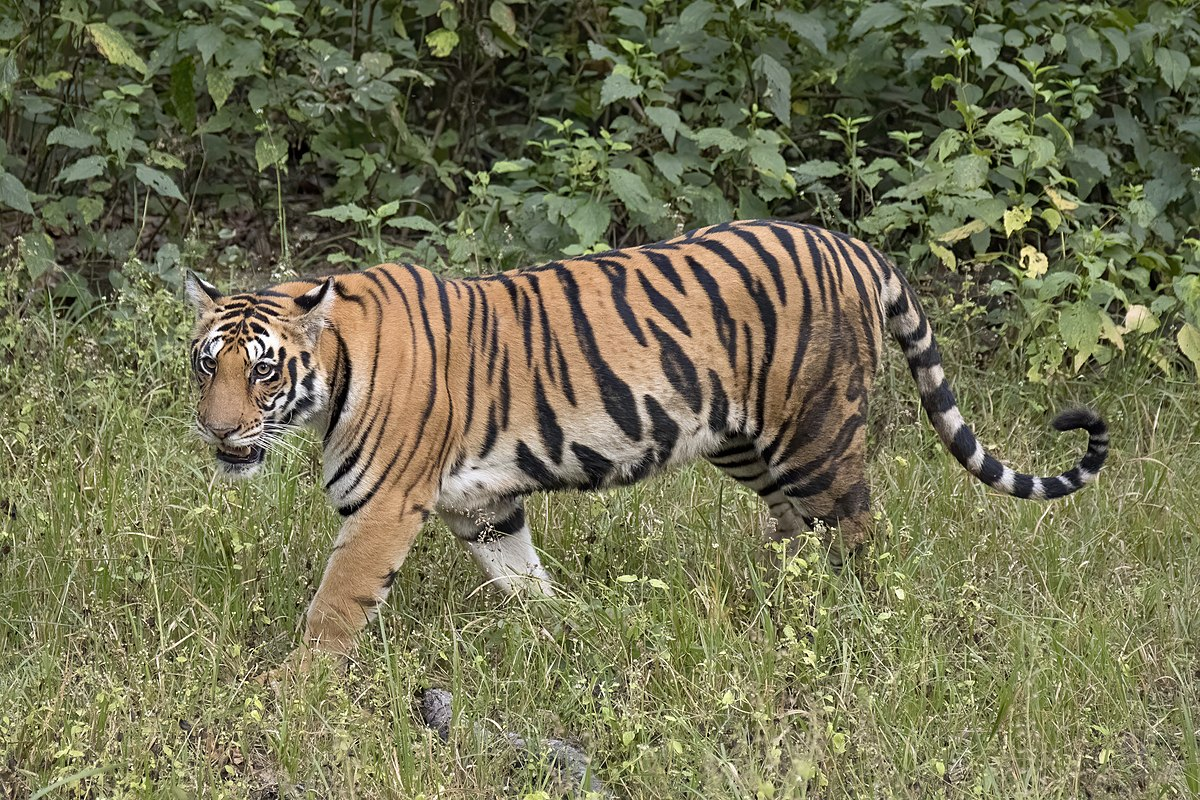
\includegraphics[width=9.37cm]{../bengalTigerWikipedia.jpg}
		\caption{Bengaalse tijger}\label{fig:benTijger}
	\end{figure}
	
\end{document}
